\documentclass{article}
\usepackage[]{geometry}
\usepackage[parfill]{parskip}
\usepackage[utf8]{inputenc}
\usepackage{graphicx}
    
\usepackage{amsmath,amssymb,amsfonts,amsthm}


\begin{document}
\pagestyle{empty}

\section*{General notes}
\begin{itemize}
\item Goal of supervised learning: predict not yet observed input
\item Motivation: ``\emph{It is probable that no universal beat tracking model exist which does not utilise a switching model to recognize style and context prior to application.}'' \cite[Collins2006]{Collins2006}
\item Instead of calculating the STFT as for input featuress discover a good set of features by representation learning. (``\emph{Learned representations often result in much better performance than can be obtained with hand-designed representations.}'' \cite[Goodfellow2016]{Goodfellow2016})
\item Common association between sequence modeling and recurrent networks: ``\emph{Given a new sequence modeling task or dataset, wich architecture should one use?}'' \cite[Bai2018]{Bai2018}
\item Certain convolutional architectures can reach state-of-the-art accuracy in audio synthesis (e.g. Google WaveNet \cite[Oord2016]{Oord2016})
\item Do TCNs outperform LSTM architectures in this particular sequence modeling task?
\item Dataset size: ``\emph{[...] a rough rule of thumb is that a supervised deep learning algorithm will gernerally achieve acceptable performance with around 5000 labeled examples per category and will match or exceed human performance when trained with a dataset containing at least 10 million labeled examples.}'' \cite[Goodfellow2016]{Goodfellow2016}
\item Contrast of the two statements:
\begin{itemize}
\item ``\emph{Feature extraction is an essential step towards efective and accurate beat/downbeat positions extraction.}'' \cite[Khadkevich2012]{Khadkevich2012}
\item ``\emph{The system shows state-of-the-art beat and downbeat tracking performance on a wide range of different musical genres and sryles. It does so ny avoiding hand-crafted features such as harmonic changes, or rhythmic patterns, but rather leans the relevant features directly from audio.}'' \cite[Boeck2016b]{Boeck2016b}
\end{itemize} 
\end{itemize}


\section{Psychoaccoustics}

\begin{itemize}
\item Experiments on the tempo sensitivity on humans have shown that the ability to notice tempo changes is proportional to the tempo, with the JND (just noticable difference) beeing around 2-5\% \cite{Drake1993}.
\end{itemize}


\section{Beat Tracking Difficulty of a Song}
It is difficult to reliably extract high-level rhythm related features from musical excerpt having properties such as [Quinton2016]
\begin{itemize}
\item absence of a clear rhythmic structure (Classical music)
\item soft onsets
\item blurred note transitions (e.g. classigal music dominated by string instruments)
\item heavy syncopation
\item expressive timing (e.g. rubato playing)
\item the problem of 'octave errors' (detecting double or half time the rate of the ground truth)
\end{itemize}
\vspace{1em}
Quantify the difficulty of beat tracking with indicators such as
\begin{itemize}
\item beat strength [Tzanetakis2002]
\item pulse clarity [Lartillot2008]
\item entropy of a cyclic tempogram [Grosche2010] as an indicator of the tempo salience  
\end{itemize}

\section{Signal processing}

\subsection{Time-Frequency Reassignment}
\begin{itemize}
\item audio signals have a distribution of energy that varies in time and frequency
\item a spectrogram is constrained by an unfortunate tradeoff between resolution in time and frequency
\item time-frequency reassignment: mapping the data to time-frequency coordinates that are nearer to the true region of support of the analyzed signal
\item time-frequency reassignment has been used in a variety of applications for obtaining improved time and frequency estimates for time-varying spectral data [cite... 16-18]
\end{itemize}


\section{Feature extraction}

\begin{itemize}
\item ``Is it important to use several features?'' [Durand2015]
\end{itemize}


\paragraph{Potential features:} Zero Crossing Rate, Energy, Danceability, Entropy of Energy, Spectral Centroid, Spectral Spread, Spectral Entropy, Spectral Flux, Spectral Roll off, MFCC, Chroma Vector, Chroma Deviation



\section{Clustering}
The whole training data gets separated in different clusters. Each cluster represents a homogenous subset of the whole data set, i.e., the multiple models are trained for specific aspects (e.g. genre, timbre, rhythmical patterns, instrumentation, etc.). 

% basic principles of how humans understand rhythms

\section{Beat Tracking System}

\begin{figure}[htbp]
\centering
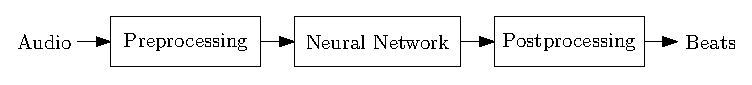
\includegraphics[scale=1.0]{figures/beat_tracking_system.eps}
\caption{Beat tracking system signal flow}
\label{fig:}
\end{figure}	

\section{Preprocessing}

\begin{itemize}
\item ``\emph{Many artificial intelligence tasks can be solved by designing the right set of features to extraxt for that task, then providing theses features to a simple machine learning algorithm.}'' \cite[Goodfellow2016]{Goodfellow2016}
\item Two different types of input features: Onset events and harmonic changes
\item Assumtion: Most harmonic changes occur inside a piece of music are located at metric bars \cite[Khadkevich2012]{Khadkevich2012}
\item in complex polyphonic mixtures of music, simultaneously occurring events of high intensities lead to masking effects that prevent any observation of an energy increase of a low intensity onset. To circumbent thesse masking effects, detection functions were proposed that analyze the signal in a bandwise fashion to extract transients occurring in certain frequency regions of the signal [Grosche2011]
\end{itemize}



The first step in the approach consists of preprocessing the original data. Data preprocessing refers to all transformations on the raw data before the resulting training set is fed to the machine learning algorithm. It includes different methods such as normalization, transformation and feature extraction. 

The data set contains raw pulse code modulated (PCM) audio signals stored as WAV files. For the sake of consistency and also to reduce computational complexity the audio signal is resampled at a sampling rate $f_s = 44.1 \,\text{kHz}$ and converted to a monaural signal by averaging both stereo channels. 


\begin{itemize}
\item Slice audio $x(t)$ into frames $x_n(t)$, $n = 1, 2,\dots, N$, where $N$ is the number of frames
\item Compute complex spectrogram $X(n,k)$ with FFT 
\item Complex spectrogram is converted to the power spectrogram $S(n, k) = |X(n, k)|^2$
\item Mel-spectrogram $M(n,m) = \log \left( S(n,k) \cdot F(m,k)^T + 1.0 \right)$
\end{itemize}
\vspace{1em}

Short-time Fourier transform:
\begin{align}
X(n,k) = \sum_{m = 0}^{N-1} w(m) \, x(m + n  h) \, e^{-2 \pi j  k /N}
\end{align} 

Spectrogram: 
\begin{align}
S(n,k) = |X(n,k)|^2
\end{align} 

Separation of magnitude and phase:
\begin{align} 
X(n,k) = |X(n,k)| \, e^{\, j \phi(n,k)}
\end{align} 


\subsection{Chroma representation}

\begin{itemize}
\item CRP (chroma DCT-reduced log-pitch) features have significant amount of robustness to changes in timbre an instrumentation \cite[Mueller2010]{Mueller2010}
\end{itemize}




\section{Machine learning model}

Seuqence-to-sequence prediction:
\begin{itemize}
\item the entire input sequence can be used to predict each output (not feasible in real time processing)
\end{itemize}

Binary classification problem:
\begin{itemize}
\item beat (class 1)
\item no beat (class 0)
\end{itemize}


\subsection{Sequence modeling}

We are given an input sequence $x_1, \dots, x_T$ and wish to predict some corresponding outputs $y_1, \dots, y_T$ at each time. The key constraint is that to predict the output $y_t$ for some time $t$, we are constrained to only use those inputs that have been previously observed: $x_1, \dots , x_t$. Formally, a seqeunce modeling network is any function $f : \mathcal X^{T} \rightarrow \mathcal Y^{T}$ that produces the mapping
\begin{align}
\hat y_1, \dots, \hat y_T = f(x_1,\dots, x_T)
\end{align}

The architecture should take a sequence of any length and map it an output seqence of any length and map it to an output sequence of the same length.

The goal of learning in the sequence modeling setting is to find a network $f$ that minimizes some expected loss between the actual outputs and the predictions, $L(y_0,\dots,y_T, f(x_0,\dots,x_T))$, where the sequences and outputs are drawn according to some distribution [Bai2018].



\subsection{Data representation}

% https://musicinformationretrieval.wordpress.com/2017/04/25/audio-beat-tracking-human-annotation-strategies/

The Beat Tracking task requires annotations in the form of time instants of beats from a musical excerpt. Additionally, the tempo, metrical level of the beat and downbeat positions can also be annotated for related tasks like downbeat tracking/ meter tracking/ tempo tracking etc.

The method for obtaining ground truth annotations depends on whether the aim is to identify descriptive beat locations or to replicate a human tapping response. In the former case, an initial estimate of the beat locations can be obtained by recording tap times for a given musical excerpt and iteratively modifying and auditing the obtained beat positions while in the latter case, the ground truth can be completely defined by the tapping response \cite{Davies2009b}.

The audio excerpt in time domain and its spectrogram can be visualised using tools like Sonic Visualizer. Beat locations can first be obtained by recording the tap locations the musical excerpt and then manually correcting these locations for exact onsets.  Annotators can also follow a semi-automatic process, for example in [2], where beats and downbeats were first obtained through the ircambeat software and then errors were manually corrected by human annotators.



\paragraph{General:}

After preprocessing the audio we obtain the observation set $ O = \left\{ \mathbf x^{(\alpha)}, \,\mathbf y_T^{(\alpha)} \right \}_{\alpha = 1}^p$, with $p$ samples in total. As elements the set cointains:
\begin{itemize}
\item feature vector: $\mathbf x \in \mathbb R^{(\text{sequence length}, \,\text{input size})}$
\item true label: $\mathbf y_T \in \{0,1, \dots, (\text{number of classes}-1)\}^{\text{(sequence length)}}$
\end{itemize}

\begin{itemize}
\item Data augmentation (transformation or adding noise) $\Rightarrow$ prediction gets robust against transformation and noisy signals
\item output: $y$ probability of beat instant per time frame 
\end{itemize}


\begin{itemize}
\item $p = 698$
\item $\mathbf x \in \mathbb R^{(3015, \,120)}$
\item $\mathbf y_T \in \{0,1\}^{(3015)}$
\end{itemize}

\subsection{Recurrent Networks (RNNs)}

% As the model class we choose a recurrent neural network as seen in Fig. 
% \begin{figure}[htbp]
% \centering
% \includegraphics[scale=1.0]{figures/recurrent_network.eps}	
% \caption{Common structure of recurrent networks.}
% \label{fig:}
% \end{figure}

\begin{figure}[htbp]
\centering
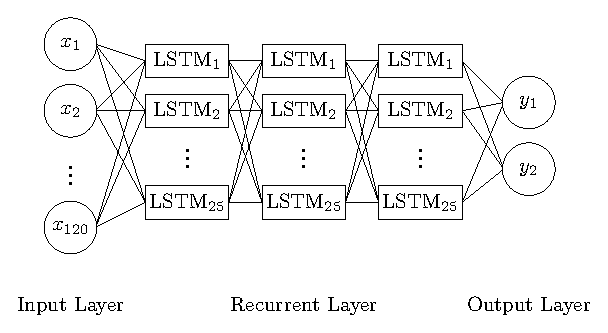
\includegraphics[scale=1.0]{figures/neural_network_boeck.eps}
\caption{Model architecture in \cite{Boeck2011}[Boeck2011]}
\label{fig:}
\end{figure}	

\subsection{Temporal Convolutional Netwoks (TCNs)}

\begin{itemize}
\item the convolutions are casual, i.e, no information leakage from future to past (compare to bidirectional RNN).
\item long effective history sizes, i.e., the ability for networks to look very far into the past to make a prediction (receptive field?), by using a combination of very deep networks (augmented with residual layers) and dilated convolutions 
\item TCNs do not use gated mechanisms 
\item TCN uses causal convolutions, i.e., convolutions where an output at time $t$ is convolved only with elements from time $t$ and earlier in the previous layer 
\item employ dilated convolutions that enable an exponentially large receptive field
\item for a 1-D sequence input $\mathbf x \in \mathbb R^T$ and a filter $f:\{ 0, \dots, k-1\} \rightarrow \mathbb R$, the delated convolution operation $F$ on element $s$ of the sequence is defined as
\begin{align}
F(s) = (\mathbf x *_d f)(s) = \sum_{i=0}^{k-1} f(i) \, \mathbf x_{s-d\,i}
\end{align}
where $d = 2^\nu$ is the delation factor, $\nu$ is the level of the network and $k$ is the filter size.  
\end{itemize}
\begin{figure}[htbp]
	\centering
	\includegraphics[]{figures/tcn_dilated_casual_convolution.pdf}
	\caption{Dilated casual convolution. Source: \cite{Bai2018}[Bai2018]}
	\label{fig:figure1}	
\end{figure}

\begin{itemize}
\item In place of a concolutional layer TCNs employ a gneric residual module. 
\item Each residual block contains a branch leading out to a series of transformations (dilated causal convolution, weight normalization, rectified linear transfer function, spatial dropout), whose outputs are added to the input $\mathbf x$ of the block
\item this allows layers to learn modifications to the identity mapping rather than the entire transformation, which has been shown to benefit deep neural networks (where?)
\item within a residual block there exist two layers of dilated causal convolution and a rectified linear unit (ReLU) \cite[Nair2010]{Nair2010} as a non-linearity
\item for normalization a weight normalization \cite[Salimans2016]{Salimans2016} is applied to the convolutional filters 
\item additionaly spatioal dropout \cite[Srivastava2014]{Srivastava2014} is added after each dilated convolution for regularization (at each training step, a whole channel is zeroed out)
\end{itemize}


\subsection{Trellis networks (TrellisNets)}
\begin{figure}[htbp]
\centering
\includegraphics[scale=1.0]{figures/trellis_net_atomic_level.pdf}
\caption{TrellisNet at an atomic level.}
\label{fig:TrellisNetAtomic}
\end{figure}	

\begin{itemize}
\item[\textbf{Input:}] $x_{1:T} = x_1, \dots, x_T, \quad x_t \in \mathbb R^p, \quad x_{1:T} \in \mathbb R^{T \times p}$ \vspace{0.5em}\\ 
with sequence length  $T$  input dimensionality  $p$
\item[\textbf{Output:}] $y_{1:T} = y_1, \dots, y_T = G(x_1, \dots, x_T)$ \vspace{0.5em} \\
with function $G: \mathcal X^T \rightarrow \mathcal Y^T$ 
\item[\textbf{Hidden:}] $z_t^{(i)} \in \mathbb R^q$
\end{itemize}




\paragraph{LogSoftmax:}

A LogSoftmax normalization is added the last layer of the neural network to obtain the log-probabilities for the differnent classes.
\begin{align}
\text{LogSoftmax}(x_i) = \log\left(\frac{\exp{(x_i)}}{\sum_j \exp(x_j)}\right)
\end{align} 



\subsection{Performance measure}

\paragraph{Loss Function}
Cross entropy is defined for two probability distributions $p$ and $q$ as
\begin{align}
H(p,q) = - \sum_{x \in \mathcal X} p(x) \log q(x).
\end{align} 
In machine learning cross entropy can be used as a loss funciton to measures the performance of a classification model. The probability $p_{i}$ is the true label (binary indicator 0 or 1), where as the distribution $q_{i}$ is the predicted value of the current model. 


\subsection{Regularization techniques}


\subsection{Optimization}

\begin{itemize}
\item Regularization with Dropout or Weight Decay
\item check out cyclical learning rates \cite{Smith2017}[Smith2017]
\end{itemize}


Estimate generalization error with a validation set during training. Stop training when the error on the validation set rises (early stopping).

\subsection{Valididation}

\paragraph{Test set method} Split the observarions into to disjunct subsets 
\begin{align*}
\text{observations}
\begin{cases}
	\text{ training data } \left\{ \left(\mathbf x^{(\alpha)}, \,\mathbf y_T^{(\alpha)}\right) \right \}, \, \alpha \in \{1,\dots, p\} & \\	
	\;\rightarrow E^T \text{ selects model parameters} & \\	 \\
	\text{ test data } \left\{ \left(\mathbf x^{(\beta)}, \,\mathbf y_T^{(\beta)}\right) \right \}, \, \beta \in \{1,\dots, q\} & \\	
	\;\rightarrow \widehat{E}^G \text{ estimates generalization error} & \\	
\end{cases}
\end{align*} 

\paragraph{n-fold cross-validation} 



\section{Postprocessing}

We use a probabilistic dynamic model to exploit the seqential structure of music, generally resulting in a more robust estimation.

As a postprocessing step we make use of a dynamic Bayesian network (DBN) which jointly infers tempo an phase of the beat.

\vspace{1em}
Hidden variables: 
\begin{itemize}
\item $\omega$ - the tempo
\item $\phi$ - the position inside the beat period
\end{itemize}

\vspace{1em}
In order to infer the hidden variables from an audio signal, we specify three entities:

\begin{itemize}
\item \textbf{transition model}: describes the transitions between the hidden variables 
\item \textbf{observation model}: takes the beat activations from the neural network
\item \textbf{initial distribution}: encodes prior knowledge about the hidden variables
\begin{itemize}
\item test probability model for given tempo estimation 
\end{itemize}
\end{itemize}

\subsection{Transition model}
\begin{itemize}
\item The number of observations $M$ per beat at tempo $T$ in BPM is defined as 
\begin{align}
M(T) = \dfrac{60}{T} \,f_r \quad \left[ \dfrac{\text{frames}}{\text{beat}}\right]
\end{align} 
\item The beat position state is dependent on the tempo by using exactly one  state per audio frame.


% \item The beat period is discretized into $\Phi = 640$ equidistant cells
\item $\Phi \in \{1,2,\dots, M(T)\}$ denotes the position inside the beat period (pib)
\item The tempo space corresponds to integer valued beat positions in the interval $[M(T_{\text{max}}), M(T_{\text{min}})]$, with 
\begin{align}
N_{\text{max}} = M(T_{\text{min}}) - M(T_{\text{max}}) + 1
\end{align} 
different tempo states.

% \item For the position inside the beat period we have the following recurrence relation
% \begin{align}
% \phi_k = (\phi_{k-1} + \omega_{k-1} -1) \mod \Phi + 1
% \end{align}  
% \item The tempo space is also discretized tempos between 56 and 216 BPM 
% \begin{align}
% \text{BPM} = \omega \times 60 \times f_r \,/ \, \Phi
% \end{align} 
\item The tempo in beat positions per time frame $\dot \Phi \in \{M(T_{\text{max}}), M(T_{\text{max}}) + 1,  \dots, M(T_{\text{min}})\}$ 
\item For example: 
\begin{align*}
T_{\text{min}} = 56 \,\text{BPM} & \;\rightarrow \; M(T_{\text{min}}) = 107 \\
T_{\text{max}} = 215 \,\text{BPM} &\;\rightarrow \; M(T_{\text{max}}) = 28 
\end{align*} 
\vspace{-1.5em}
\begin{align*}
&\Phi \in \{1, 2, \dots ,107\} \\
&\dot \Phi \in \{28, 29, \dots ,107\}
\end{align*} 


\item Transitions to each tempo is allowed but only at beat times
\begin{align}
\omega_k = 
\begin{cases}
\omega_{k-1}, & P(\omega_k|\omega_{k-1}) = 1 - p_\omega \\
\omega_{k-1}+1, & P(\omega_k|\omega_{k-1}) = \frac{p_\omega}{2} \\
\omega_{k-1}-1, & P(\omega_k|\omega_{k-1}) = \frac{p_\omega}{2} \\
\end{cases}
\end{align} 
\item The probability of tempo change is heuristically set to $p_\omega = 0.002$
\end{itemize}


\subsection{Observation model}


\section{Evaluation}


\subsection{Performance measures}

Set of annotated beat times $\mathcal A = \{a_1, \dots, a_A\}$ \\
Set of predicted beat times $\mathcal B = \{b_1, \dots, b_B\}$ \\

True positive if beat is in $\pm 70\,\text{ms}$ rage of annotated beat

$tp =$ number of true positives \\
$fp =$ number of false positives (extra detections) \\
$fn =$ number of false negatives (missed detections) 

\paragraph{Precision and recall:} $ $

$\text{precision} = \dfrac{tp}{tp + fp}\;, \qquad \text{recall} = \dfrac{tp}{tp + fn}$


\paragraph{F-measure:} $ $

$F_1 = 2 \cdot \dfrac{\text{precision} \cdot \text{recall}}{\text{precision} + \text{recall}} = \dfrac{2\, tp}{2\, tp + fp + fn}$

\paragraph{P-score:} Define two sequences $T_a$ and $T_b$ as 

$T_a(n) = \begin{cases}
	1, &\text{ if } n \in \mathcal A \\
	0 , & \text{ otherwise }
\end{cases}, \qquad T_b(n) = \begin{cases}
	1, &\text{ if } n \in \mathcal B \\
	0 , & \text{ otherwise }
\end{cases}$

$\text{P-score} = \dfrac{\displaystyle \sum_{m=-w}^w  \sum_{n}\,  T_a(n)\,  T_b(n+m)}{\max(A,B)} \;, \qquad \text{where } w = 0.2 \, \text{median}(\Delta_a)$ 







% \subsection{Network training}

% \begin{figure}[htbp]
% \centering
% \includegraphics[scale=0.6]{figures/loss_bs-10_fold_0.eps}
% \caption{Loss function for 30 epechs with batch size 30 and learning rate $10^{-4}
% $}
% \label{fig:loss}
% \end{figure}	

% \begin{figure}[htbp]
% \centering
% \includegraphics[scale=0.6]{figures/loss_bs-100_w-70__fold-1.eps}
% \caption{Loss function for 30 epechs with batch size 100 and learning rate $10^{-4}
% $}
% \label{fig:loss}
% \end{figure}	


\section{Appendix}

\subsection{Hyperparameter} 
\begin{itemize}
\item window function (e.g. Hamming window)
\end{itemize}


\bibliographystyle{unsrt}
\bibliography{references}

\end{document}